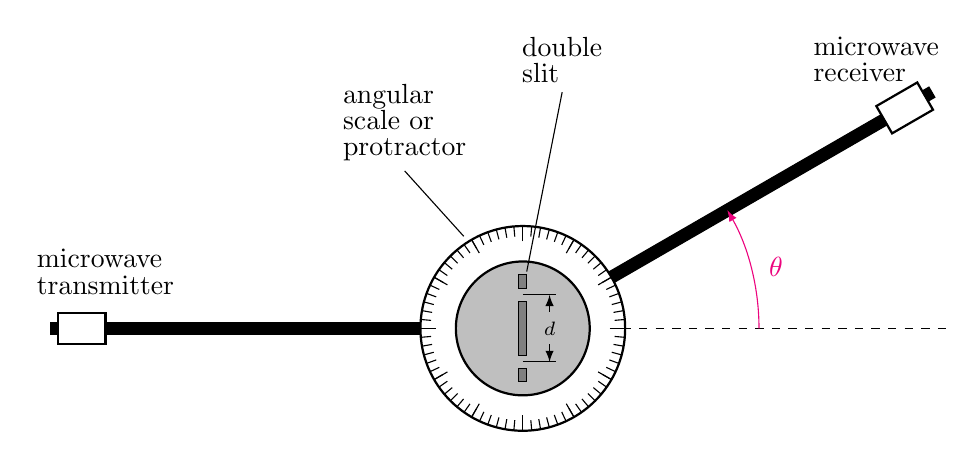
\begin{tikzpicture}
    % Setup dimensions
    \def\L{6}         % screen-slit distance
    \def\t{0.075}     % support beam thickness
    \def\ts{0.05}     % slit thickness
    \def\len{0.6}     % transmitter/receiver length
    \def\wid{0.2}     % transmitter/receiver width
    \def\Rbg{1.3}     % outer radius of the angular scale
    \def\Rsm{0.85}    % inner radius of the angular scale
    %
    % Transmitter arm
    \draw[fill=black] (-\L,-\t) rectangle (0,\t);
    \draw[thick, fill=white] (-\L+0.5*\wid,-\wid) rectangle (-\L+0.5*\wid+\len,\wid) node[above=3, align=left] {microwave\\[-0.25em]transmitter};
    \draw[dashed] (0,0) -- (0.9*\L,0);
    %
    % Receiver arm
    \begin{scope}[rotate around={30:(0,0)}]
        \draw[fill=black] (0,-\t) rectangle (\L,\t);
        \draw[thick, fill=white] (\L-0.5*\wid,-\wid) rectangle
        (\L-0.5*\wid-\len,\wid) node[above=5, align=left] {microwave\\[-0.25em]receiver};
    \end{scope}
    %
    % Angular table
    \draw[thick, fill=white] (0,0) circle (\Rbg);
    \foreach \th in {0, 5, ..., 360}
        \draw[rotate around={\th:(0,0)}] (0.9*\Rbg, 0) -- (\Rbg, 0);
    \foreach \th in {0, 30, ..., 360}
        \draw[rotate around={\th:(0,0)}] (0.85*\Rbg, 0) -- (\Rbg, 0);
    \draw[thick, fill=gray!50] (0,0) circle (\Rsm);
    %
    % Double slit
    \draw[fill=gray] (-\ts, 0.6*\Rsm) rectangle (\ts, 0.8*\Rsm);
    \draw[fill=gray] (-\ts, -0.4*\Rsm) rectangle (\ts, 0.4*\Rsm);
    \draw[fill=gray] (-\ts, -0.6*\Rsm) rectangle (\ts, -0.8*\Rsm);
    \draw (0, -0.5*\Rsm) -- (0.5*\Rsm, -0.5*\Rsm);
    \draw (0,  0.5*\Rsm) -- (0.5*\Rsm,  0.5*\Rsm);
    \draw[latex-latex] (0.4*\Rsm, -0.5*\Rsm) -- (0.4*\Rsm, 0.5*\Rsm) node[pos=0.5, fill=gray!50] {\scriptsize $d$};
    %
    % Labels
    \draw (\ts, 0.85*\Rsm) -- (0.5,3) node[above, align=left] {double\\[-0.25em]slit};
    \draw (-0.75, 0.9*\Rbg) -- (-1.5,2) node[above, align=left] {angular\\[-0.25em]scale or\\[-0.25em]protractor};
    \draw[-latex, RubineRed] (0.5*\L, 0) arc[start angle=0, end angle=30, radius=0.5*\L] node[right=3, pos=0.5] {$\theta$};
\end{tikzpicture}